\newpage
%%%%%%%%%%%%%%%%%%%%%%%%%%%%----->SECCIÓN 2<-----%%%%%%%%%%%%%%%%%%%%%%%%%
\chapter{Rayos cósmicos}
%%%%%%%%%%%%%%%%%% NEWWWW
Los rayos cósmicos (en adelante CR por sus siglas en inglés) son partículas cargadas que viajan a través del espacio intergaláctico a velocidades cercanas a la luz. Estas partículas, que provienen de diversas fuentes, incluyendo el Sol, supernovas, pulsares, agujeros negros entre otras, son en su mayoría protones y núcleos atómicos. Su composición es diversa, con una predominancia de protones $(~89\%)$, seguidos por núcleos de helio $( 10\%)$ y núcleos pesados $( 1\%)$. También pueden estar constituidos por partículas elementales como electrones o fotones de alta energía  (\cite{kampert_2012}).

En este capítulo, nos adentraremos en el estudio de los rayos cósmicos, comenzando con una descripción de su origen y el espectro de energías que presentan. Describiremos en detalle los mecanismos de detección de los rayos cósmicos, proporcionando una visión de cómo estos fenómenos astrofísicos son estudiados en la actualidad.  A continuación, exploraremos cómo se propagan a través de la heliósfera, el campo geomagnético y finalmente la atmósfera terrestre. En cada etapa de su viaje, los rayos cósmicos interactúan con el medio de formas que afectan su propagación y finalmente su detección en la Tierra.

Finalmente describiremos la morfología de las cascadas aéreas extensas producidas en la atmósfera terrestre y las interacciones hadrónicas y electromagnéticas que las generan. Este análisis es esencial, ya que nuestro estudio se centra en la detección en tierra de la componente electromagnética de las cascadas aéreas, especialmente los muones y electrones que llegan al nivel del suelo. Estas partículas subatómicas juegan un papel crucial en nuestra comprensión de los rayos cósmicos y su interacción con la atmósfera terrestre. 

\section{Origen y espectro de energías}

Los rayos cósmicos, que abarcan un amplio espectro energético, son en su mayoría hadrones, partículas subatómicas que incluyen protones y núcleos atómicos. Estos hadrones cubren valores inferiores a $1 GeV$ hasta más allá de $10^{20} eV$.  A baja energía, la detección de estos hadrones está limitada por la existencia de un corte geomagnético, al menos en medidas realizadas cerca de la Tierra (\cite{Riggi_2023}). El flujo de hadrones de baja energía está sujeto a grandes variaciones temporales, tanto periódicas como transitorias, debido a la influencia del Sol. Sin embargo, estas variaciones se vuelven despreciables a medida que aumenta la energía cinética de los primarios.

Para la medición se pueden emplear diferentes métodos, que dependen de la energía de las partículas. Los métodos directos de detección de rayos cósmicos implican el uso de instrumentos enviados al espacio en globos, cohetes o satélites para medir las características de las partículas primarias que llegan a la Tierra. Algunos ejemplos de estos instrumentos incluyen los detectores de trazas nucleares, que muestran las trayectorias de las partículas cargadas; los espectrógrafos magnéticos, que aplican campos magnéticos para desviar las trayectorias de las partículas cargadas; los calorímetros, que calculan la energía que pierden las partículas cargadas \cite{tomassetti_2023}.

Un ejemplo representativo de un instrumento de detección directa es el Espectrómetro Magnético Alfa (AMS) en la Estación Espacial Internacional, que mide los rayos cósmicos de alta energía o el Espectrómetro de Isótopos de Rayos Cósmicos (CRIS) en la nave espacial Advanced Composition Explorer (ACE) (\cite{tomassetti_2023}), que proporciona mediciones de los isótopos de núcleos de rayos cósmicos galácticos que van desde el helio hasta el zinc.

Los métodos indirectos de detección utilizan la atmósfera como un calorímetro y detectan las partículas secundarias que se crean cuando las partículas primarias chocan con la atmósfera. Estas partículas secundarias son más abundantes y más fáciles de detectar que las partículas primarias. Uno de los instrumentos más representativos de detección indirecta es el Observatorio Pierre Auger, que utiliza una técnica de detección híbrida para estudiar los rayos cósmicos de ultra alta energía y sondear las interacciones hadrónicas a energías mucho más allá de las accesibles por los aceleradores de partículas (\cite{engel_2021}) (los detalles se describirán en el capítulo 2).

El espectro energético de los rayos cósmicos, obtenido a través de toda esta variedad de instrumentos y experimentos, muestra tendencias notables como la rodilla, la segunda rodilla y el tobillo, que corresponden a cambios abruptos en la pendiente a un valor de energía específico. Este espectro sigue una ley de potencia, del tipo $E^{-\gamma}$, con el exponente $\gamma$ variando en diferentes regiones energéticas (\cite{Riggi_2023}). Para visualizar mejor la tendencia del espectro, se suelen representar los valores de flujo multiplicados por $E^{\gamma}$, eligiendo un valor adecuado del exponente $\gamma$ (entre 2,5 y 3) como se observa en la figura \ref{fig:spectrum}. Esta representación permite verificar si la tendencia de los datos sigue esta ley, ya que idealmente los valores se dispondrían a lo largo de una línea horizontal.

\begin{figure}
    \centering
    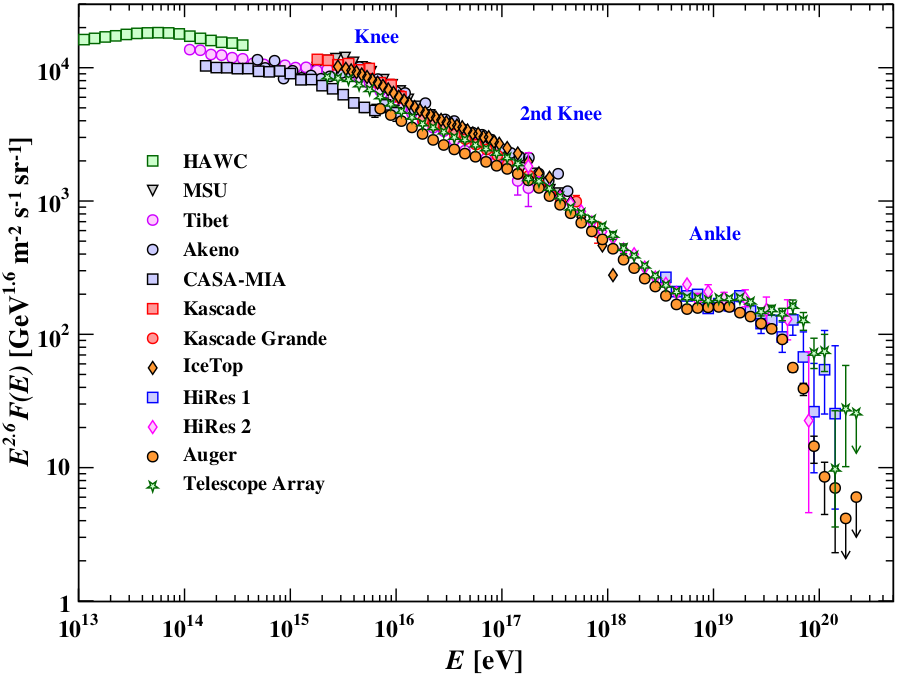
\includegraphics[width=0.8\linewidth]{Figs/CR_spectrum.png}
    \caption{Enter Caption. Fuente \cite{PDG}}
    \label{fig:spectrum}
\end{figure}

%%%%%%  ORIGEN DE LOS RAYOS CÓSMICOS DE ANTES DEL TOBILLO Y DESPUÉS DEL TOBILLO.
%%%% Pierre Cristofari (The transition From Galactic to Extragalactic cosmic rays)
Se tiene evidencia de que los rayos cósmicos (CR) de energías inferiores a la "rodilla" del espectro energético son de origen galáctico. Esto se basa en la observación de los rayos gamma del disco galáctico, que se espera que emitan una señal de rayos gamma mejorada (un incremento en la emisión) debido a la interacción de los CR con el material interestelar (\cite{Cristofari_2023}). Sin embargo, cuando la energía de los CR supera cierto umbral, conocido como el "tobillo", la fuente es de origen extragaláctico (\cite{augerextra}). Esta transición se debe a que los CR de alta energía no pueden confinarse dentro de la galaxia cuando su radio de Larmor es mayor que el tamaño típico del halo galáctico.

\section{Propagación de CR a través de la heliósfera}

El Sol, debido a su proximidad y características, se ha convertido en un laboratorio esencial para la comprensión de la física estelar y es fundamental para la investigación en física del plasma y astrofísica (\cite{Rozelot_2006}). %%%%%ROZELOT

\begin{figure}
    \centering
    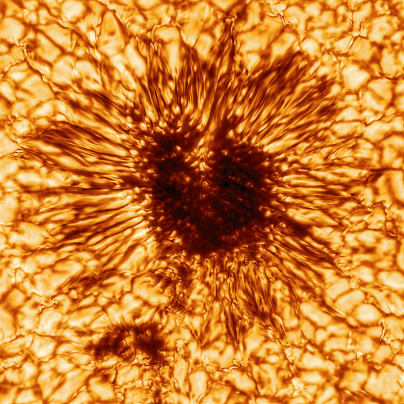
\includegraphics[width=0.6\linewidth]{Figs/sunspot_small.png}
    \caption{La cámara Inouye Solar Wave Front Correction (WFC) de la NSF capturó su primera imagen de una mancha solar el 28 de enero de 2020. La imagen revela un corte de la estructura tridimensional de la mancha solar, que se forma por la convergencia de campos magnéticos intensos y gas caliente que burbujea desde abajo. Aunque la imagen presenta una paleta de colores cálidos con tonos rojos y naranjas, fue tomada por el visor contextual de la Cámara de Campo Amplio del Telescopio Solar Inouye a una longitud de onda de 530 nanómetros, que corresponde a la parte amarillo verdosa del espectro visible. Crédito: NSO/AURA/NSF}
    \label{fig:sunspotNSO}
\end{figure}

 %aunque considerado una estrella común
Todos los estudios del Sol hasta la fecha han revelado la sorprendente diversidad de su campo magnético, que se concentra en pequeños tubos de flujo magnético de alta intensidad que emergen desde el interior del Sol y causan estructuras magnéticas retorcidas en la corona (\cite{schrijver_2009}). Adicionalmente, se ha obtenido información muy detallada sobre su estructura interna: delimitada por distintas capas, cada una de ellas fundamental en la generación y difusión de su energía. La zona interna del Sol, que incluye el núcleo y la zona radiativa, abarca aproximadamente el $85\%$ del radio total. El núcleo, que es donde ocurre la fusión nuclear, se encuentra dentro del $20\%$ del radio solar y contiene el $34\%$ de la masa del Sol. Por encima del núcleo, la zona radiativa se extiende desde aproximadamente el $25\%$ hasta el $70\%$ del radio solar. Por lo tanto, la mayor parte del Sol está compuesta por su zona interna (\cite{Hanslmeier_2023}). 

El  casi$~30\%$ restante le corresponde a la zona convectiva. En esta zona, el Sol no es lo suficientemente caliente para transferir energía por radiación térmica. En esta capa Sol presenta una estructura conocida como granulación, para transportar energía desde el borde de la zona radiativa hasta la superficie. A medida que el plasma se eleva, libera calor al llegar a la superficie solar. Luego, al enfriarse, desciende, perpetuando un ciclo continuo de transporte de energía. Este proceso genera campos magnéticos a través de un mecanismo conocido como 'mecanismo de dínamo solar (\cite{Sturrock_1986}).

La atmósfera del Sol, que incluye la fotosfera, la cromosfera y la corona, juega un papel crucial en la actividad solar. Aunque estas capas representan una pequeña fracción del radio total del Sol ($0.43\%$), son el escenario de varios fenómenos que definen la actividad solar. La fotosfera, que es la capa que vemos desde la Tierra y tiene un grosor de aproximadamente 500 km, es donde se manifiestan las manchas solares, que son indicadores de la actividad magnética del Sol y su mecanismo de convección. La cromosfera, con un grosor de aproximadamente 2500 km, es el lugar donde ocurren las fulguraciones solares, que son explosiones de energía causadas por el reajuste de las líneas del campo magnético. La corona solar, aunque se extiende mucho más allá de la cromosfera, es notablemente menos densa y es la fuente del viento solar (\cite{Rozelot_2006}). Estos fenómenos están intrínsecamente vinculados al campo magnético del Sol, que parece ser el principal impulsor de las actividades solares (\cite{Sturrock_1986}). Así, aunque la atmósfera del Sol representa solo una pequeña fracción de su radio total, su influencia se extiende mucho más allá, afectando no solo al clima espacial, sino también a nuestra vida diaria en la Tierra.

Más allá de la los límites de lo que se puede denominar corona solar, se extiende la heliósfera: una región extensa dominada por el Sol, caracterizada por el viento solar y el campo magnético solar. Esta región protege nuestro sistema solar de la mayoría de los rayos cósmicos galácticos y de los vientos interestelares. El límite de la heliosfera, conocido como heliopausa, se forma cuando el viento solar interactúa con el medio interestelar (\cite{schrijver_2009}). Esta interacción resulta en una compleja dinámica de campos magnéticos y partículas energéticas. El estudio de la heliosfera es esencial para entender el entorno cósmico que nuestro sistema solar atraviesa y para ampliar nuestro conocimiento de otros procesos astrofísicos.

El viento solar, compuesto principalmente por electrones y protones, se origina en la corona solar y se expande hacia el exterior a velocidades de entre 300 y 800 kilómetros por segundo. Este flujo arrastra el campo magnético del Sol, formando una estructura helicoidal conocida como espiral Parker (\cite{Rozelot_2006}). Las fluctuaciones en la velocidad y densidad del viento solar afectan al campo magnético interplanetario y contribuyen a los fenómenos de meteorología espacial (\cite{Rozelot_2006}). El estudio del viento solar es esencial para entender la interacción entre el Sol y su entorno cósmico, y para arrojar luz sobre los procesos que rigen la morfología de la heliosfera.
%%%%%%%%%%%
Las sondas espaciales dan la oportunidad de medir directamente parámetros físicos fundamentales del viento solar. El viento solar no es un fluido estacionario: continuas fluctuaciones del campo magnético son producidas por movimientos turbulentos del gas en el Sol, y escapan hacia el medio interplanetario. Discontinuidades en el campo magnético y ondas de choque se producen por la colisión de viento solar lento y viento solar rápido y por erupciones en la corona solar, eyecciones de masa coronal (CME) y fulguraciones. Las CMEs se propagan a través del sistema solar, y pueden ser medidas cerca de la Tierra como eyecciones de masa coronal interplanetarias (ICMEs). Cuando son suficientemente rápidas generan una onda de choque delante de ellas como se observa en la figura \ref{icme}.

La figura \ref{CME_2003} muestra un ejemplo de una fulguración intensa y una CME, que perturban considerablemente la Heliosfera. Las imágenes fueron tomadas por diferentes instrumentos a bordo de la nave SOHO (ESA/NASA) el 28 de octubre de 2003  y la CME alcanzó la Tierra un día más tarde: grupos de manchas (arriba a la izquierda) indican intensa actividad y complejas estructuras magnéticas en la superficie solar. En la mayor y más compleja de esas regiones aparecieron brillantes fulguraciones. Fue observado, por ejemplo, por el telescopio de ultravioleta extremo (EIT; arriba a la derecha de la figura). Una CME rápida y grande fue observada unos minutos más tarde por el coronógrafo LASCO (al fondo de la figura), propagándose por la corona a una velocidad de 1000 km/s.

\begin{figure}[H]
    \centering
    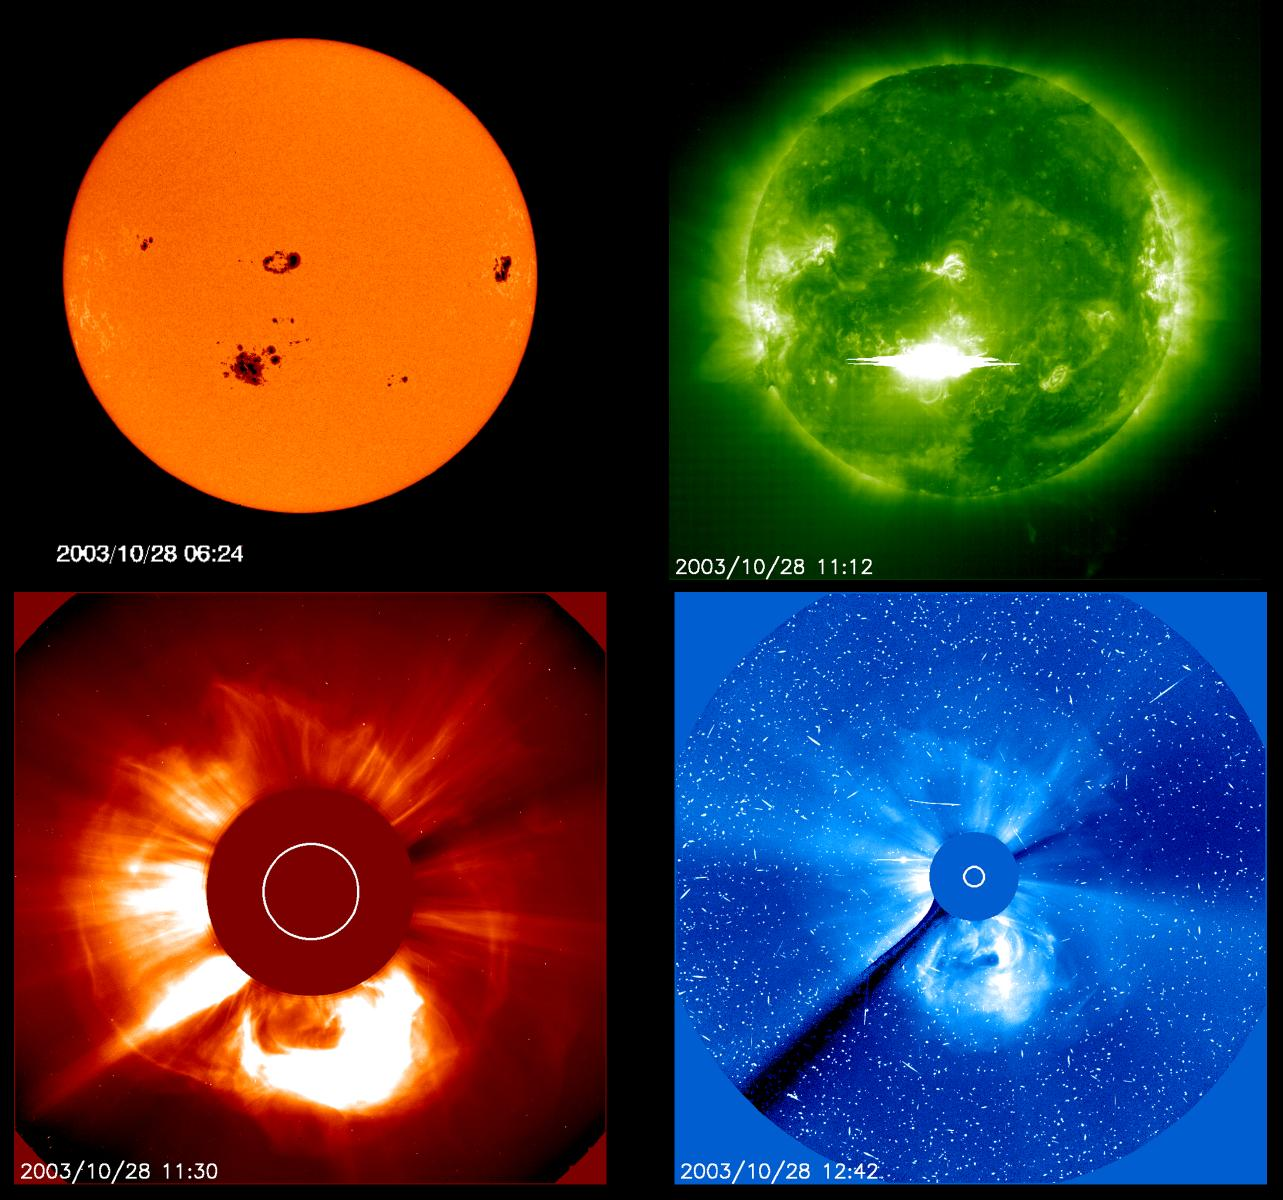
\includegraphics[width=0.6\linewidth]{Figs/flare_2003-10-28.jpg}
    \caption{Enter Caption. Fuente SOHO/MDI, SOHO/EIT, SOHO/LASCO (ESA/NASA)}
    \label{CME_2003}
\end{figure}

La figura \ref{imce} ilustra esquemáticamente este fenómeno: la estructura magnética expulsada desde la corona (línea roja) perturba el campo magnético heliosférico (líneas azules). El viento solar no puede penetrar en la ICME, por lo que se comprime junto con el campo magnético, o se desvía alrededor de la ICME, como indican las dos flechas azules. La configuración de las líneas de campo cambia. En la interfaz entre la ICME y el viento solar circundante, el campo magnético se vuelve turbulento. En esta heliosfera perturbada, tanto los rayos cósmicos solares como los galácticos experimentan condiciones de propagación muy diferentes a las de la heliósfera en estado tranquilo (\cite{NMDB}).

\begin{figure}[H]
    \centering
    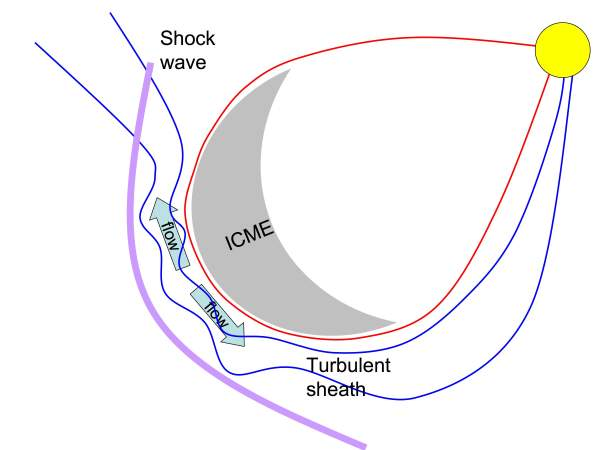
\includegraphics[width=0.5\linewidth]{Figs/Dessin_ICME_sm_0.jpg}
    \caption{Enter Caption. Fuente \cite{NMDB}}
    \label{imce}
\end{figure}
Cuando los rayos cósmicos galácticos llegan a la heliósfera, interactúan con el viento solar que afecta de diferente manera a los rayos cósmicos según su energía. Los que tienen una energía muy alta, $>10GeV$,  tienen una trayectoria rectilínea, ya que la fuerza de Lorentz que ejerce el campo magnético es despreciable en comparación con su momento lineal. Las partículas de energía moderada, de unos pocos $GeV$, tienen una trayectoria difusiva. La difusión se produce por la presencia de irregularidades en el campo magnético del viento solar, que provocan cambios en la dirección e intensidad del campo a lo largo de la trayectoria de las partículas. Estos cambios se deben a la turbulencia del plasma, que genera fluctuaciones en el campo magnético a diferentes escalas espaciales y temporales. La difusión de los rayos cósmicos de energía moderada implica una pérdida de información sobre su dirección de origen y una modulación de su flujo en función del ciclo solar.
%%%%%%%%% NEW

El ciclo solar es el periodo de 11 años en el que la actividad solar varía de forma periódica. Esto se manifiesta en el conteo de manchas solares. El número de manchas solares se correlaciona inversamente con el flujo de rayos cósmicos galácticos medido por la red de monitores de neutrones en la Tierra (más detalles en el capítulo 3). Esto se debe a que cuando el número de manchas solares es alto, el viento solar es más fuerte y el campo magnético interplanetario es más turbulento, lo que dispersa más a los rayos cósmicos galácticos y reduce su flujo. Por el contrario, cuando el número de manchas solares es bajo, el viento solar es más débil y el campo magnético interplanetario es más regular, lo que dispersa menos a los rayos cósmicos galácticos y aumenta su flujo.

Además de la modulación de 11 años, los rayos cósmicos galácticos también presentan variaciones de menor amplitud y duración, relacionadas con la rotación solar de 27 días y con la localización de las regiones activas en el Sol. Estas variaciones se deben a que el viento solar y el campo magnético interplanetario no son homogéneos ni isotrópicos, sino que dependen de la latitud y la longitud solar. Así, los rayos cósmicos galácticos experimentan cambios en su flujo, su espectro de energía y su anisotropía, que es la distribución angular de su intensidad.

Otro aspecto importante del ciclo solar es que cada 11 años el campo magnético solar invierte su polaridad, lo que implica que el ciclo completo es de 22 años. Esto afecta a la propagación de los rayos cósmicos galácticos en la Heliósfera, ya que el campo magnético interplanetario tiene una configuración diferente según la polaridad del campo magnético solar. De esta forma, el flujo de rayos cósmicos galácticos tiene una forma distinta en dos ciclos solares consecutivos. En uno, el flujo tiene un pico pronunciado, con un máximo claro, mientras que en el otro, el flujo tiene una forma más plana, con un máximo menos definido. Escalas superiores al ciclo solar de 11 años quedan por fuera de los alcances de este trabajo.

\textbf{Decrecimientos Forbush}:  La modulación de los rayos cósmicos por el viento solar se ve afectada por la presencia de ICMEs, que son estructuras complejas y dinámicas de plasma y campo magnético que se originan en el Sol y que se propagan por la Heliosfera. La figura \ref{forbush}  muestra este fenómeno  registrado en mayo de 2005 por el observatorio Pierre Auger y el monitor de neutrones de Los Cerrillos (Chile).  Se observa que el flujo de rayos cósmicos disminuye hasta un 20\% durante el paso de una ICME. Estos eventos se denominan decrementos de Forbush, en honor al físico de rayos cósmicos Scott Forbush, que los descubrió en 1937.

\begin{figure}[H]
    \centering
    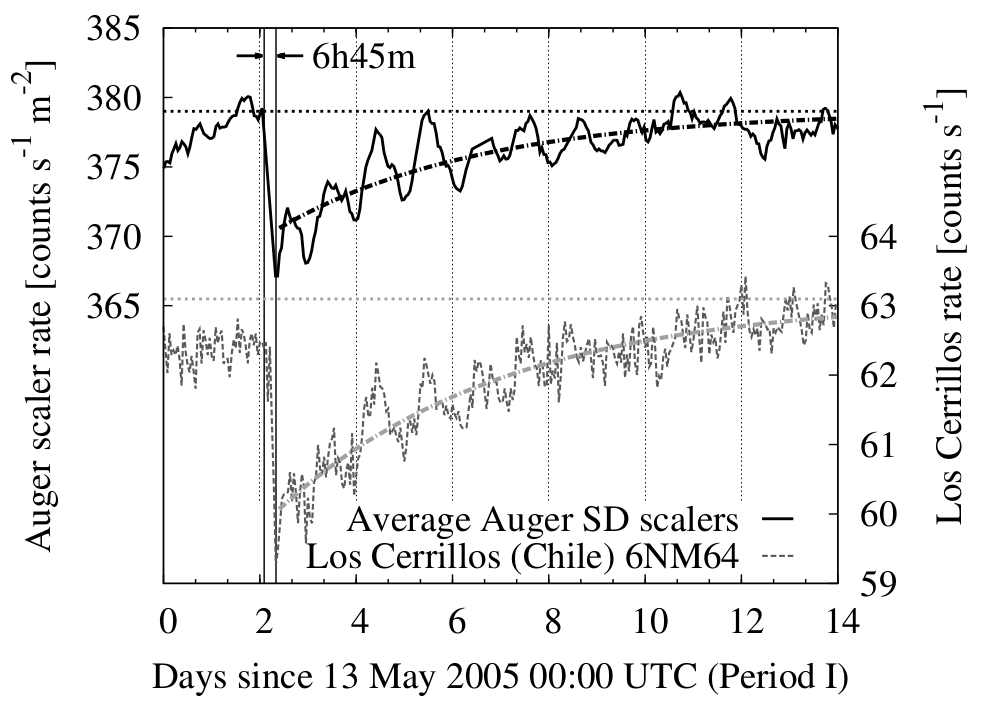
\includegraphics[width=0.6\linewidth]{Figs/mauro_forbush.png}
    \caption{Enter Caption. Fuente \cite{asorey}}
    \label{forbush}
\end{figure}

La disminución del flujo de rayos cósmicos se debe al efecto de apantallamiento que produce la estructura magnética de la ICME y la onda de choque que la acompaña (figura \ref{imce}). El campo magnético de la ICME es más intenso y turbulento que el del viento solar, lo que dispersa más a los rayos cósmicos y los desvía de su trayectoria original. Además, la onda de choque de la ICME comprime el plasma y el campo magnético, lo que crea una barrera que dificulta el paso de los rayos cósmicos. Estos efectos son más notorios para las partículas de menor energía, que son más sensibles a la fuerza de Lorentz que ejerce el campo magnético. Así, los rayos cósmicos que atraviesan una ICME sufren una modulación de su flujo, su espectro de energía y su anisotropía.

\section{Propagación de CR a través del Campo Geomagnético}

Al llegar al entorno terrestre, los rayos cósmicos galácticos se ven afectados por el campo magnético terrestre y la atmósfera. El campo magnético terrestre modula el flujo de los rayos cósmicos galácticos, que depende de su energía y de su dirección de llegada. Los rayos cósmicos galácticos de baja energía son más sensibles a la fuerza de Lorentz que ejerce el campo magnético y pueden ser desviados o excluidos de la magnetosfera. Los rayos cósmicos galácticos de alta energía pueden penetrar la magnetosfera y llegar a la atmósfera.

La Tierra tiene un campo magnético generado por las corrientes eléctricas de su núcleo, que tiene una forma aproximada de un dipolo, con dos polos magnéticos cerca de los polos geográficos. El campo magnético terrestre no está aislado, sino que interactúa con el viento solar, que es el plasma que sale del Sol y que tiene un campo magnético. El viento solar comprime el campo magnético terrestre en la dirección del Sol y lo estira en la dirección opuesta, creando una cola magnética. El campo magnético terrestre forma un sistema casi cerrado de líneas de campo, que delimitan una región del espacio donde el campo magnético terrestre domina sobre el campo magnético interplanetario. Esta región se llama magnetosfera y tiene una forma asimétrica, como se muestra en la figura [1]. La magnetosfera protege a la Tierra de la radiación solar y de los rayos cósmicos galácticos de baja energía, pero también permite la entrada de partículas cargadas que producen fenómenos como las auroras.


\section{Propagación de CR a través de la atmósfera terrestre}

Cuando los CR primarios llegan a la atmósfera terrestre, chocan con los átomos del aire y producen una lluvia de partículas secundarias, que tienen menos energía que el primario. Algunas de estas partículas pueden decaer o interactuar nuevamente con el aire, generando más partículas secundarias. Este proceso se repite varias veces hasta que la energía del primario se disipa o se alcanza el nivel del suelo. A este fenómeno se le llama cascada aérea extensa (en adelante EAS, por sus siglas en inglés).

El estudio de las EAS es fundamental para entender el origen, la naturaleza y la distribución de los CR. Sin embargo, la detección directa se puede realizar hasta el rango de aproximadamente $10^{15}eV$. Como son absorbidos por la atmósfera, deben medirse mediante globos, cohetes o satélites con los que se puede determinar la energía, la composición de la partícula y la dirección de incidencia. Para energías mayores a $10^{15}$ eV, la detección se hace primordialmente de forma indirecta debido a que se reduce significativamente el número de partículas que arriban a la Tierra como se muestra en la figura (\ref{fig:spectrum}). Para tal fin se utilizan detectores a nivel del suelo que registran las señales que dejan las partículas secundarias de las EAS. Estos detectores pueden medir la intensidad, la dirección, la composición y la energía de las EAS, y a partir de ahí inferir las propiedades de los CR primarios \cite{kampert_2012}. 

Para analizar las EAS, se necesita conocer cómo interactúan las partículas con la atmósfera. Un parámetro importante es la profundidad atmosférica $X$ (\ref{eq:eq2}), que mide la cantidad de materia que atraviesa una partícula primaria en su camino por la atmósfera. La profundidad atmosférica depende de la altura $h$ sobre el nivel del mar y de la densidad del aire $\rho(h)$.  
\begin{equation}
X_{v}= \int_{h}^{\infty} \rho (h') dh'.
\label{eq:eq2}
\end{equation}
Por otra parte, teniendo en cuenta la naturaleza de las partículas secundarias, se pueden identificar tres componentes principales: la componente electromagnética, que está conformada por electrones, positrones y fotones; la componente hadrónica, constituida de piones, kaones y bariones, y la componente muónica, generada por el decaimiento de piones y kaones cargados. La figura \ref{fig:fig3} ilustra los procesos de interacción mostrados anteriormente y cómo éstos generan cada una de las componentes. Estas tres componentes se generan debido a interacciones electromagnéticas y hadrónicas en el proceso de penetración a través de la atmósfera que describiremos con un poco más de detalle a continuación.

\begin{figure}[htb!]
\centering
    \begin{center}
        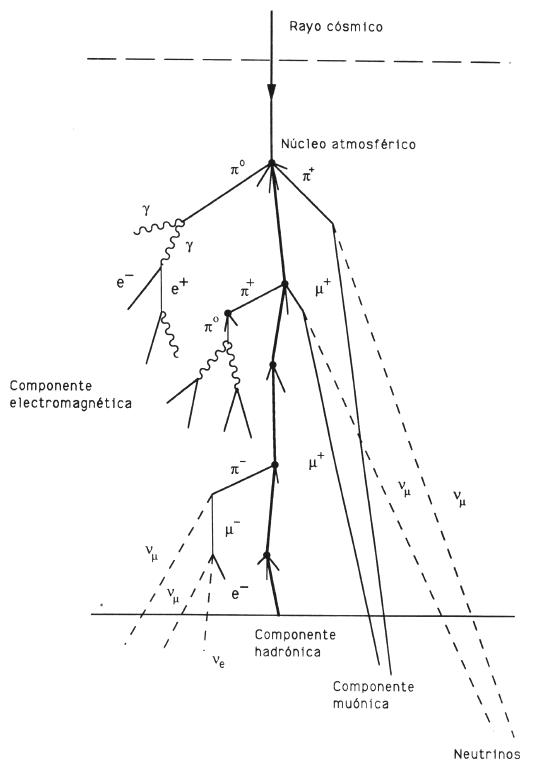
\includegraphics[width=0.5\textwidth]{Figs/componentes_cas.jpg}
    \end{center}{}
    \caption[Esquema del desarrollo de una EAS iniciada por un hadrón.]{Esquema del desarrollo más probable de una EAS iniciada por un hadrón \cite{mauro:tesis}. En la figura se observa el decaimiento del hadrón en piones cargados y neutros, y estos a su vez, al decaer, generan fotones, electrones y muones. Se identifican tres componentes: electromagnética, muónica y hadrónica.}
    \label{fig:fig3}
\end{figure}

\subsection{Interacciones electromagnéticas}
Están presentes cuando el primario incidente es un fotón o un electrón, los principales canales de interacción son la producción de pares y radiación de frenado. Estas partículas pueden crear o emitir otras partículas del mismo tipo al interactuar con los átomos del aire. Los fotones pueden crear pares de electrones y positrones, y estos pueden emitir más fotones al frenarse (bremsstranhlung). Este proceso se detiene cuando los fotones tienen una energía de 1.02 MeV. Para un núcleo de aire con carga $Z$ y número atómico $A$, los procesos de producción son:
\begin{equation}
\begin{split}
&Bremsstrahlung\quad e \quad \xrightarrow{Y^{A}_{Z}} \quad e\gamma ,  \quad y \\
&Pares \quad \gamma \xrightarrow{Y^{A}_{Z}} \quad e^{+}e^{-} \\
\end{split}
\end{equation} 

Otros procesos electromagnéticos que influyen en esta pérdida de energía y deben ser considerados son la\textbf{pérdida de energía por Ionización} de una partícula cargada que atraviesa la materia con un espesor $\lambda$ que es descrita por la ecuación de Bethe-Bloch:
\begin{equation}
dE_{i} = \frac{\lambda \gamma^{2}z^{2}}{\gamma^{2}-1}\kappa_{1}(ln(\gamma^{2}-1)- \beta^{2}+\kappa_{2})
\label{eq:eq20}
\end{equation}

Donde $\beta = v/c $ es la velocidad de la partícula en unidades de la velocidad de la luz, $\gamma$ es el factor de Lorentz, $z$ es la carga de la partícula ionizada en unidades de $e$. Las dos constantes $\kappa_{1}= 0.153287 MeV g^{-1}$ y $\kappa_{2}= 9.386417 MeV g^{-1}$ son los valores correspondientes para el aire \cite{Heck1998}. Esta expresión es usada para calcular la perdida por energía de ionización a través de la trayectoria de la partícula. Por ejemplo, la pérdida de energía de muones como función de su energía está representado en la figura \ref{fig:fig4}.\\

\begin{figure}[htb!]
\centering
        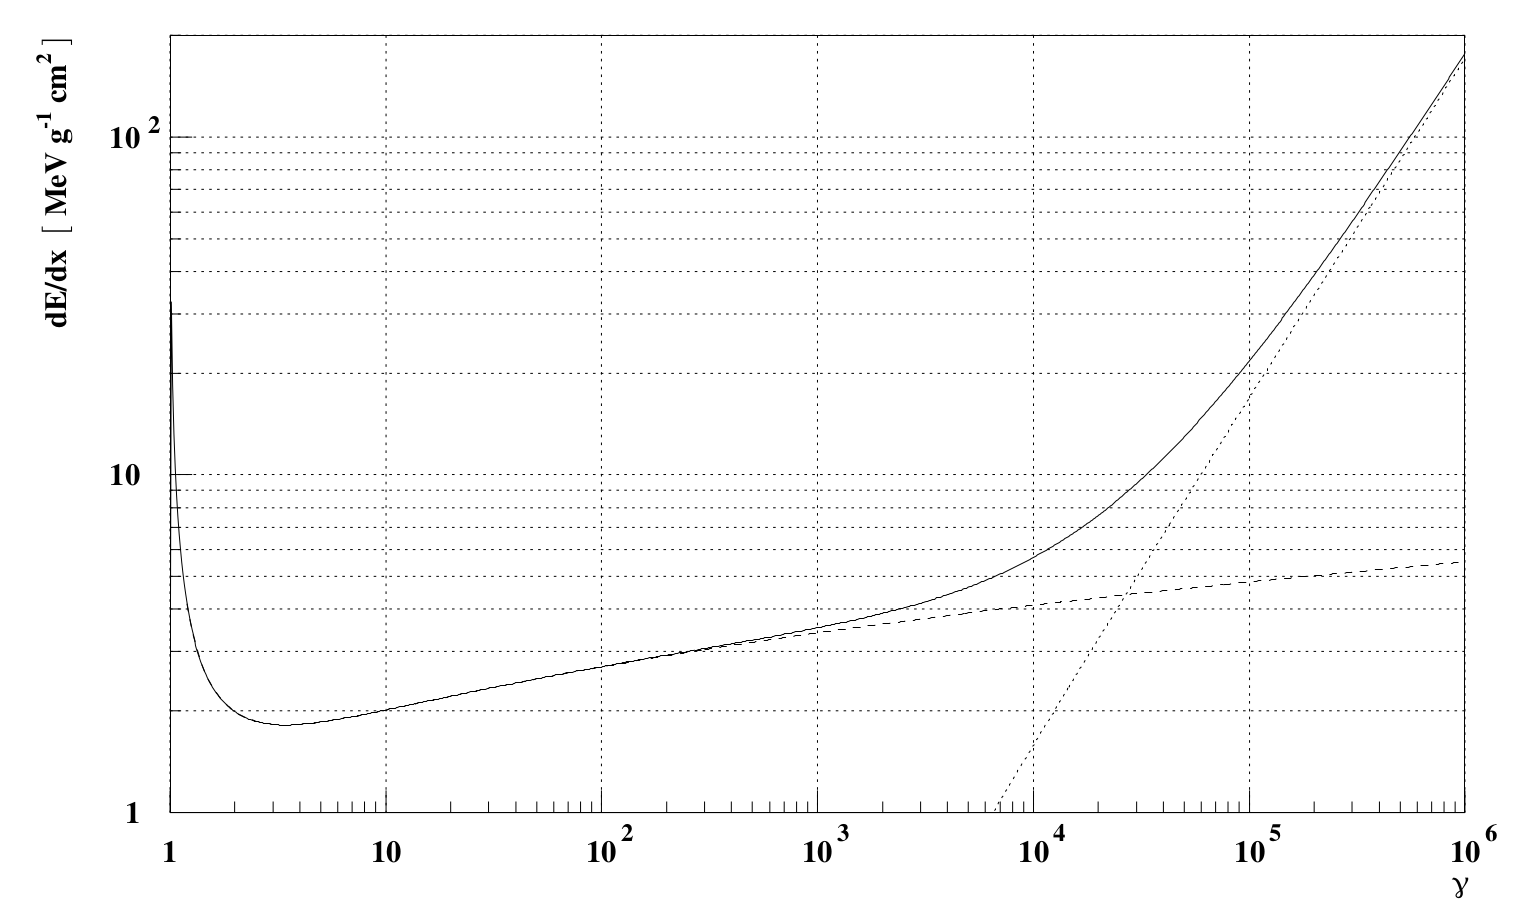
\includegraphics[width=0.7\textwidth]{Figs/Bethe_Muons.png}
        \caption[Ecuación de Bethe-Bloch para los muones.]{Pérdida de energía de Muones en el aire como función del factor de Lorentz \cite{Heck1998}. Están indicadas las contribuciones de la ionización (línea seccionada) y la producción de pares (línea punteada).}
        \label{fig:fig4}
\end{figure}

La \textbf{Dispersión múltiple de Coulomb} que ocurre cuando las partículas cargadas son dispersadas por el campo eléctrico Coulombiano de los núcleos de aire. Allí la dirección de propagación es alterada pero no cambia la energía de la partícula. La distribución angular de esta dispersión es descrita por la teoría de Moliére (\cite{Heck1998}).  

\subsection{Interacciones hadrónicas}
%%%%% NEW
Las interacciones hadrónicas son un componente fundamental en el estudio de las lluvias atmosféricas extensas (EAS). Aunque la cromodinámica cuántica (QCD) proporciona una base sólida para entender las interacciones fuertes, los procesos con múltiples partículas producidas en las interacciones hadrónicas aún no pueden ser calculados con precisión. Para superar esta limitación, se han desarrollado modelos que hacen suposiciones adicionales y utilizan parametrizaciones fenomenológicas y empíricas (\cite{Allen}).

Estos modelos son esenciales para interpretar las EAS y deben estar optimizados para un amplio rango de energías. Además, es crucial que se actualicen constantemente a medida que se obtienen más datos de los aceleradores o de grandes instrumentos como el Observatorio Pierre Auger \cite{andrada_2021}. Las interacciones hadrónicas generan piones cargados y neutros ($\pi^{-},\pi^{+},\pi^{0}$), así como kaones, que tienen una tendencia mayor a decaer que a interactuar. Los canales de decaimiento más probables para estas partículas son los siguientes:
\begin{equation*}
\pi^{0} \rightarrow \gamma\gamma \quad [{98.823 \pm 0.034}{\%}] \quad y
\end{equation*}

\begin{equation}
\pi^{0} \rightarrow e^{+}e^{-} \gamma \quad [{1.174 \pm 0.035}{\%}] .
\end{equation}

\begin{equation*}
\pi^{+} \rightarrow \mu^{+}\nu_{\mu} \quad [{99.98 \pm 0.00004}{\%}] \quad y
\end{equation*}
%
\begin{equation}
\pi^{-} \rightarrow \mu^{-}\nu_{\mu} \quad [{99.98 \pm 0.00004}{\%}] .
\end{equation}

\begin{equation*}
K^{+} \rightarrow \mu^{+}\nu_{\mu} \quad [{63.56 \pm 0.11}{\%}],
\end{equation*}
%
\begin{equation}
K^{+} \rightarrow \pi^{0}e^{+}\nu_{e} \quad [{5.07 \pm 0.004}{\%}],
\end{equation}
%
\begin{equation*}
K^{+} \rightarrow \pi^{+}\pi^{0} \quad [{20.67 \pm 0.08}{\%}] \quad y
\end{equation*}
%
\begin{equation*}
K^{+} \rightarrow \pi^{+}\pi^{+}\pi^{-} \quad [{5.583 \pm 0.024}{\%}] .
\end{equation*}
Que contribuyen a la componente electromagnética y muónica de las EAS. Más específicamente, componente muónica en las EAS es de particular interés debido a las propiedades relativistas de los muones y su larga vida media. Esta componente ofrece una visión directa de las primeras interacciones hadrónicas y las propiedades del hadrón inicial. Los muones de alta energía desencadenan sub-cascadas electromagnéticas y hadrónicas en la lluvia a través de interacciones tipo:
\begin{equation}
\mu^{\pm} \quad \xrightarrow{Y^{A}_{Z}} \quad \mu^{\pm}e^{+}e^{-},
\end{equation}
\begin{equation}
\mu^{\pm} \quad \xrightarrow{Y^{A}_{Z}} \quad \mu^{\pm} + hadrones.
\end{equation}